\item Find the mutual inductance in the arrangement, when a small circular loop of wire of radius ‘R’ is placed inside a large square loop of wire of side L (L>>R). The loops are coplanar and their centres coincide:
    \begin{center}
        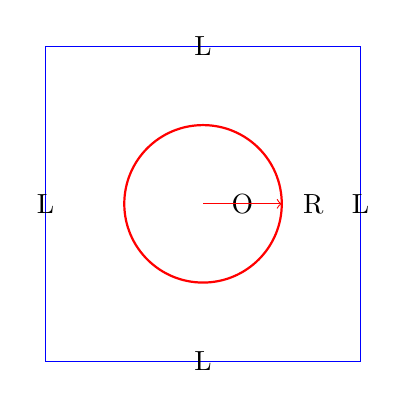
\begin{tikzpicture}
            \draw[blue] (0, 0) rectangle (4, 4);
            \draw[red, thick] (2, 2) circle (1);
            \node at (0, 2) {L};
            \node at (4, 2) {L};
            \node at (2, 0) {L};
            \node at (2, 4) {L};
            \node at (2.5, 2) {O};
            \draw[red, ->] (2, 2) -- (3, 2);
            \node at (3.4, 2) {R};
        \end{tikzpicture}
    \end{center}
    \begin{tasks}(2)
        \task $\displaystyle M = \frac{\sqrt{2} \mu_0 R^2}{L}$
        \task $\displaystyle M = \frac{\sqrt{2} \mu_0 R}{L^2}$
        \task $\displaystyle M = \frac{2 \sqrt{2} \mu_0 R^2}{L}$
        \task $\displaystyle M = \frac{2 \sqrt{2} \mu_0 R}{L^2}$
    \end{tasks}